%% 1-page TLDR: Why You Need Nonlinear Arithmetic for Barrier Certificates
\documentclass[10pt,a4paper]{article}
\usepackage[utf8]{inputenc}
\usepackage[T1]{fontenc}
\usepackage{amsmath,amssymb}
\usepackage{tikz}
\usetikzlibrary{positioning,arrows.meta,shapes.geometric,calc}
\usepackage{geometry}
\usepackage{enumitem}
\usepackage{xcolor}
\usepackage{mdframed}
\usepackage{pgfplots}
\pgfplotsset{compat=1.18}
\geometry{margin=0.7in,top=0.55in,bottom=0.55in}
\pagestyle{empty}
\setlength{\parindent}{0pt}
\setlength{\parskip}{3pt}

\newcommand{\Init}{\operatorname{Init}}
\newcommand{\Trans}{\operatorname{Trans}}
\newcommand{\Unsafe}{\operatorname{Unsafe}}

\begin{document}

\begin{center}
{\Large\bfseries Why You Need Nonlinear Arithmetic: A Barrier Certificate Example}\\[2pt]
{\small\itshape A division-by-zero safety proof where no linear invariant exists, but a quadratic barrier succeeds}
\end{center}

\vspace{-4pt}
\hrule height 0.6pt
\vspace{5pt}

\textbf{1.\ The Code.}\;
A rotation loop followed by a division.  Is \texttt{1/(x*x + y*y)} safe from \texttt{ZeroDivisionError}?

\vspace{-2pt}
{\small\ttfamily
\begin{tabbing}
xxxx\=xxxx\=\kill
def process\_after\_rotation(x, y, n):\hfill\textcolor{gray}{\# precondition: x*x + y*y >= 1}\\
\>c, s = 3/5, 4/5\hfill\textcolor{gray}{\# 3-4-5 rotation (c\textsuperscript{2}+s\textsuperscript{2}=1)}\\
\>for \_ in range(n):\\
\>\>x, y = c*x - s*y, s*x + c*y\hfill\textcolor{blue!60}{\# rotation preserves x\textsuperscript{2}+y\textsuperscript{2}}\\
\>return 1.0 / (x*x + y*y)\hfill\textcolor{red!70}{\# DIV\_ZERO if x=y=0}
\end{tabbing}}

\vspace{-4pt}
\textbf{2.\ Transition System.}

\vspace{1pt}
\begin{tabular}{@{}rl@{}}
\textbf{State:} & $s = (x, y) \in \mathbb{R}^2$ \\
\textbf{Initial:} & $\Init = \{(x,y) : x^2 + y^2 \geq 1\}$ \\
\textbf{Transition:} & $(x,y) \mapsto (cx - sy,\; sx + cy)$ \quad where $c^2 + s^2 = 1$ \\
\textbf{Unsafe:} & $\Unsafe = \{(0,0)\}$
\end{tabular}

\vspace{3pt}
\begin{minipage}[t]{0.52\textwidth}
\begin{mdframed}[linecolor=red!60,backgroundcolor=red!4,roundcorner=2pt,linewidth=0.7pt]
\textbf{3.\ Why linear arithmetic cannot work.}

\vspace{1pt}
Any linear invariant has the form $ax + by \geq c$, which defines a
\emph{halfplane}.  But $\Init$ is the \emph{exterior of a disk}---it
wraps around the origin in every direction.

\vspace{2pt}
\emph{No halfplane can contain the entire unit circle while excluding
the origin.}  Pick any $ax + by \geq c > 0$; then the point
$(-a/\!\sqrt{a^2\!+\!b^2},\, -b/\!\sqrt{a^2\!+\!b^2})$ is on the
unit circle but violates the inequality.

\vspace{2pt}
This means: \textbf{interval analysis} (boxes), \textbf{octagon
domains}, \textbf{linear template invariants}, and any technique
restricted to linear arithmetic will \emph{either} miss the invariant
(report a false positive) \emph{or} fail to prove safety.
\end{mdframed}
\end{minipage}%
\hfill
\begin{minipage}[t]{0.45\textwidth}
\vspace{-2pt}
\begin{center}
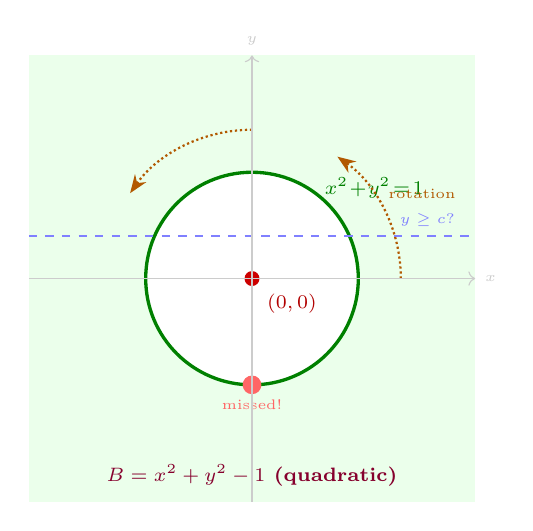
\begin{tikzpicture}[scale=1.35]
  % Safe region (exterior of circle)
  \fill[green!8] (-2.1,-2.1) rectangle (2.1,2.1);
  \fill[white] (0,0) circle (1);
  % Unit circle
  \draw[green!50!black, very thick] (0,0) circle (1);
  \node[green!50!black, font=\scriptsize] at (1.15,0.85) {$x^2\!+\!y^2\!=\!1$};
  % Unsafe point
  \fill[red!80!black] (0,0) circle (2pt);
  \node[red!70!black, font=\scriptsize, below right] at (0.05,-0.05) {$(0,0)$};
  % Failed linear barrier
  \draw[blue!50, thick, dashed] (-2.1, 0.4) -- (2.1, 0.4);
  \node[blue!50, font=\tiny] at (1.65, 0.55) {$y \geq c$?};
  % The point it misses
  \fill[red!60] (0,-1) circle (2.5pt);
  \node[red!60, font=\tiny, below] at (0,-1.05) {missed!};
  % Rotation arrows
  \draw[-Stealth, orange!70!black, thick, densely dotted]
    (1.4, 0) arc[start angle=0, end angle=55, radius=1.4];
  \draw[-Stealth, orange!70!black, thick, densely dotted]
    (0, 1.4) arc[start angle=90, end angle=145, radius=1.4];
  \node[orange!70!black, font=\tiny] at (1.6, 0.8) {rotation};
  % Quadratic barrier label
  \node[purple!70!black, font=\scriptsize\bfseries] at (0, -1.85)
    {$B = x^2 + y^2 - 1$ (quadratic)};
  % Axes
  \draw[gray!40, thin, ->] (-2.1,0) -- (2.1,0) node[right,font=\tiny]{$x$};
  \draw[gray!40, thin, ->] (0,-2.1) -- (0,2.1) node[above,font=\tiny]{$y$};
\end{tikzpicture}
\end{center}
\vspace{-4pt}
{\scriptsize The dashed blue line (linear) excludes the origin but misses
$(0,-1)$ on the unit circle.  The green circle (quadratic) separates
perfectly.  \textbf{Legend:} green = safe \& reachable ($B \geq 0$),
white interior = unreachable ($B < 0$), red dot = unsafe.}
\end{minipage}

\vspace{5pt}
\textbf{4.\ The Quadratic Barrier Certificate.}\quad
$\boxed{B(x,y) = x^2 + y^2 - 1}$

\vspace{3pt}
{\renewcommand{\arraystretch}{1.25}
\begin{tabular}{@{}rll@{}}
\textbf{Init:} & $x^2\!+\!y^2 \geq 1$
  & $\Rightarrow\; B = x^2\!+\!y^2 - 1 \geq 0$ \;\checkmark \\
\textbf{Inductive:} & $x' = cx-sy,\; y' = sx+cy$
  & $\Rightarrow\; x'^2\!+\!y'^2 = (c^2\!+\!s^2)(x^2\!+\!y^2) = x^2\!+\!y^2$ \\
  & & so $B(s') = B(s) \geq 0$ \;\checkmark \\
\textbf{Unsafe:} & $x = y = 0$
  & $\Rightarrow\; B = -1 < 0$ \;\checkmark
\end{tabular}}

\vspace{5pt}
\textbf{SOS certificate.}\;
Let $g = x^2+y^2-1$ so that $\Init = \{g \geq 0\}$.
\begin{itemize}[nosep,leftmargin=1.5em]
\item \emph{Non-negativity on} $\Init$:\;
  $B = \underbrace{1}_{\in\,\Sigma^2} \cdot\, g$
  \quad(Putinar representation with SOS multiplier $\sigma_1 = 1^2$)
\item \emph{Inductiveness}:\;
  $B(s') - B(s) = 0 = 0^2 \in \Sigma^2$
\item \emph{Separation}:\;
  $-B\big|_{\Unsafe} = 1 = 1^2 \in \Sigma^2$
\end{itemize}

\vspace{3pt}
\textbf{5.\ The punchline.}

The invariant $x^2 + y^2 \geq 1$ is preserved by rotation and violated only at the origin.
It is \emph{inherently degree 2}: no conjunction of linear inequalities $\{a_ix + b_iy \geq c_i\}$
can describe the exterior of a circle.

\textbf{All} purely-linear techniques---intervals, octagons, polyhedra, linear templates,
CEGAR with linear predicates---provably cannot verify this program.
SOS/SDP barrier synthesis exists precisely for these cases.

\end{document}
